\documentclass{beamer}
\usepackage{tikz}
\setbeamertemplate{background}{
    \begin{tikzpicture}[remember picture,overlay]
        \node[at=(current page.center)] {
            
\includegraphics[width=\paperwidth,height=\paperheight]{pic/tkkc-logo-bg.pdf}
        };
    \end{tikzpicture}
}
\usepackage{ctex, hyperref}
\usepackage[T1]{fontenc}
\usepackage{latexsym,amsmath,xcolor,multicol,booktabs,calligra}
\usepackage{graphicx,pstricks,listings,stackengine}
\usepackage{pgfplots}
\pgfplotsset{compat=1.18}
\usepackage{subfigure}
\usepackage{tcolorbox}
\usepackage{algorithm}
\usepackage{algorithmic}

\author{杨熙承 22030531}
\title{人工智能大作业演示报告}
\subtitle{}
\institute{常州工学院~~计信院}
\date{\today}
\usepackage{Tsinghua}

\definecolor{deepblue}{rgb}{0,0,0.5}
\definecolor{deepred}{rgb}{0.6,0,0}
\definecolor{deepgreen}{rgb}{0,0.5,0}
\definecolor{halfgray}{gray}{0.55}
\definecolor{commentgray}{gray}{0.45}

\lstdefinestyle{pythonstyle}{
    language=Python,
    basicstyle=\ttfamily\small,
    keywordstyle=\bfseries\color{deepblue},
    emphstyle=\ttfamily\color{deepred},
    stringstyle=\color{deepgreen},
    commentstyle=\color{commentgray},
    numbers=left,
    numberstyle=\tiny\color{halfgray},
    numbersep=5pt,
    rulesepcolor=\color{red!20!green!20!blue!20},
    frame=shadowbox,
    showstringspaces=false,
    breaklines=true
}

\lstset{
    basicstyle=\ttfamily\small,
    keywordstyle=\bfseries\color{deepblue},
    emphstyle=\ttfamily\color{deepred},
    stringstyle=\color{deepgreen},
    numbers=left,
    numberstyle=\small\color{halfgray},
    rulesepcolor=\color{red!20!green!20!blue!20},
    frame=shadowbox,
}

\begin{document}

\kaishu
\begin{frame}
    \titlepage
    % \begin{figure}[htpb]
    %     \begin{center}
    %         
\includegraphics[width=0.2\linewidth]{pic/czu.png}
    %     \end{center}
    % \end{figure}
\end{frame}

\begin{frame}
    \tableofcontents[sectionstyle=show,subsectionstyle=show/shaded/hide,subsubsectionstyle=show/shaded/hide]
\end{frame}

% 正文部分的框架
\section{有监督学习}

\begin{frame}{数据集介绍}
    \vspace{-0.5cm}
    \begin{figure}
        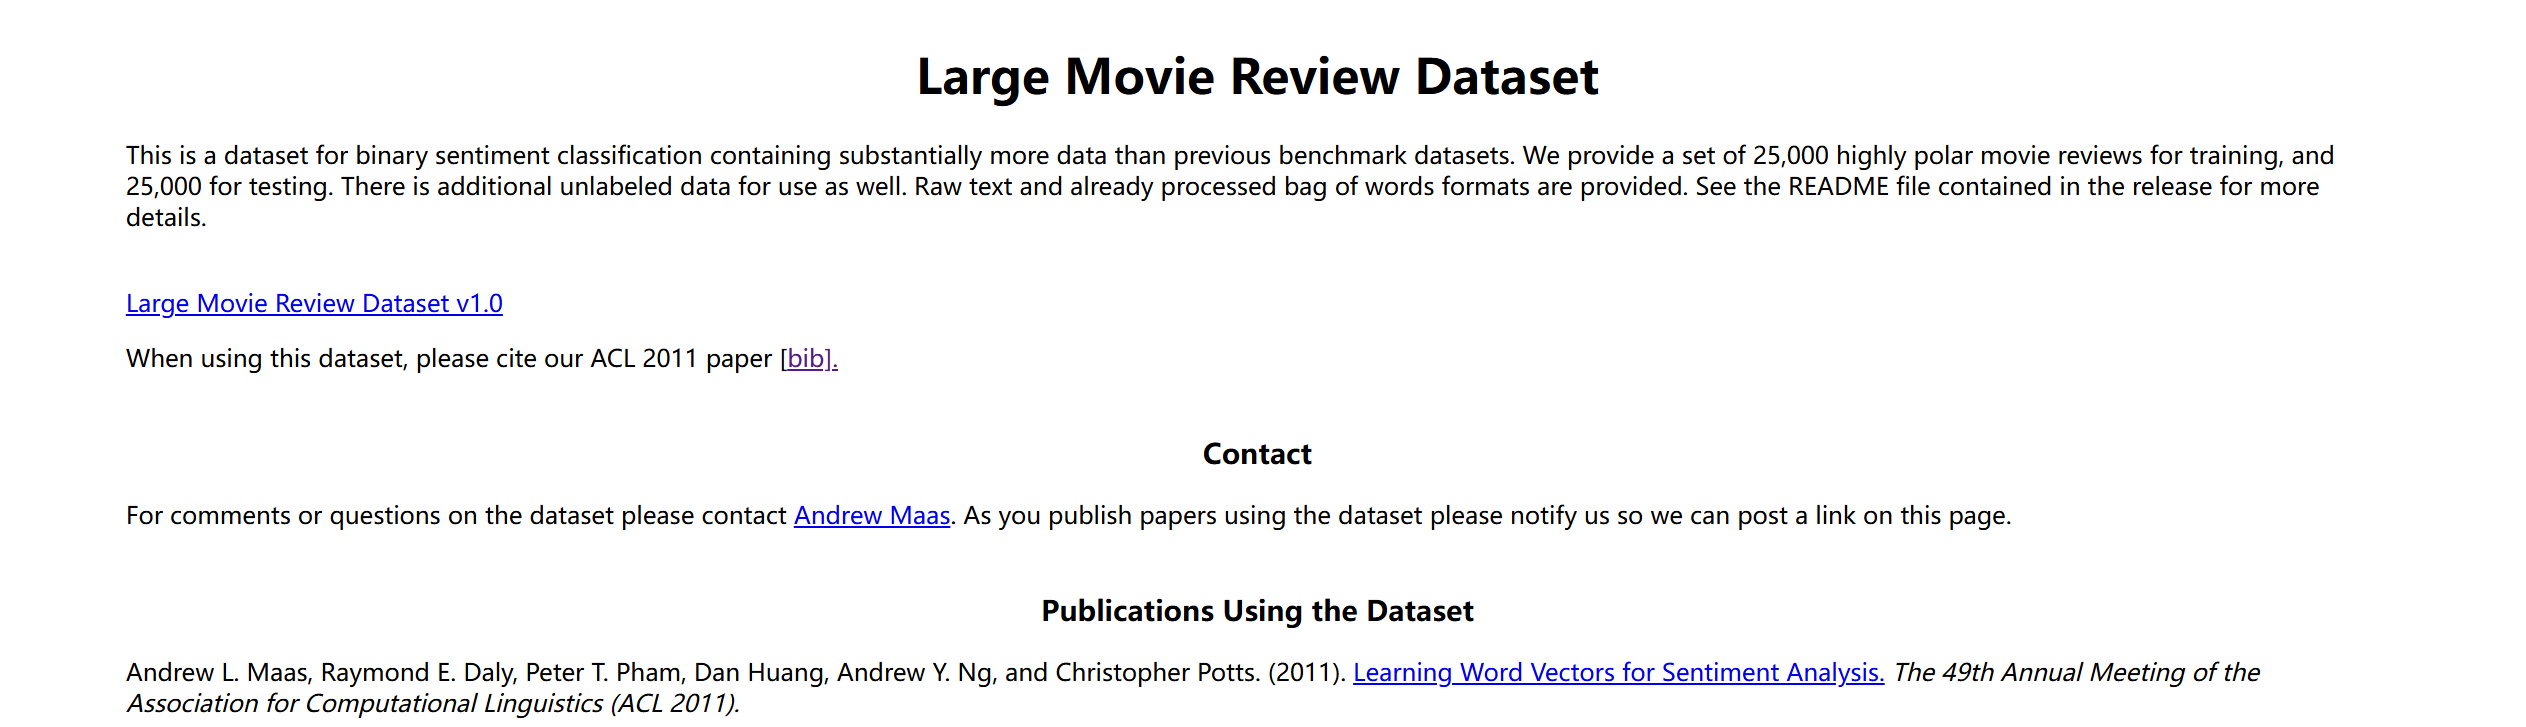
\includegraphics[width=\textwidth]{pic/stanford.png}
        \centering
    \end{figure}
    
    \begin{enumerate}
        \item Large Movie Review Dataset (IMDB)
        \item 斯坦福官方数据,训练集和测试集各25,000条电影评论
        \item data/aclImdb
        \begin{itemize}
            \item \texttt{train/}: 训练集 (pos/neg)
            \item \texttt{test/}: 测试集 (pos/neg)
        \end{itemize}
    \end{enumerate}
\end{frame}

\begin{frame}{特征工程——词频矩阵}
    \begin{columns}
        \hspace{0.7cm}
        \column{0.5\textwidth}
        \textbf{原始文本}
        \begin{enumerate}
            \item "Dr.Liu always smlies."
            \item "Dr.Liu encourages us."
            \item "Dr.Liu study harduous."
        \end{enumerate}

        \column{0.7\textwidth}
        \textbf{词汇表} \\
        \vspace{0.2cm}
        \begin{tabular}{lc||lc}
            \hline \hline
            单词 & 索引 & 单词 & 索引 \\
            \hline
            dr & 1 & smlies & 5\\
            liu & 4 & encourages & 2\\
            always & 0 & us & 7\\
            study & 6 & harduous & 3\\
            \hline
        \end{tabular}
    \end{columns}

    \vspace{0.5cm}
    \textbf{词频矩阵(Bag of Words)}
    \[
    \begin{bmatrix}
        1 & 0 & 0 & 0 & 0 & 1 & 0 & 0 & 0 & \cdots \\
        0 & 1 & 0 & 0 & 1 & 1 & 0 & 1 & 1 & \cdots \\
        0 & 1 & 1 & 1 & 0 & 0 & 1 & 0 & 0 & \cdots
    \end{bmatrix}
    \]
\end{frame}

\begin{frame}[fragile]{特征工程——Scapy、停用词、N-gram}
    \begin{columns}
        \column{0.45\textwidth}
        \textbf{词形还原 (Spacy)}
        \begin{enumerate}
            \item running $\rightarrow$ run
            \item better $\rightarrow$ good
            \item studies $\rightarrow$ study
        \end{enumerate}
        \vspace{0.5cm}
        \textbf{停用词 \& 最小文档频率}
        \begin{enumerate}
            \item 移除常见词:a, an, the...
            \item min\_df = 6:至少出现6次
        \end{enumerate}

        \column{0.55\textwidth}
        \textbf{N-gram特征}
        \begin{enumerate}
            \item 单词组合:1-2个词
            \item "very good", "not bad"
        \end{enumerate}

        \vspace{0.7cm}
        \textbf{核心代码}
        \begin{lstlisting}[style=pythonstyle, basicstyle=\tiny]
        // core code
        tfidf_spacy = TfidfVectorizer(
            tokenizer=tokenizer_spacy,
            min_df=6,
            stop_words="english",
            ngram_range=(1, 2))
        \end{lstlisting}
    \end{columns}
\end{frame}

\begin{frame}{特征工程——TF-IDF}
    \centering
    \begin{tcolorbox}[colback=white!98!black,
                      colframe=black!50,
                      width=0.9\textwidth,
                      arc=0mm,
                      boxsep=2pt]
        \begin{equation*}
            TF(t,d) = \frac{\text{词项}t\text{在文档中的次数}}{\text{文档中的总词数}}
        \end{equation*}
    \end{tcolorbox}
    
    \vspace{0.2cm}
    \begin{tcolorbox}[colback=green!10,
                      colframe=black!50,
                      width=0.9\textwidth,
                      arc=0mm,
                      boxsep=2pt]
        \begin{equation*}
            IDF(t,D) = \log_e\frac{\text{文档总数}}{\text{包含词项}t\text{的文档数}}
        \end{equation*}
    \end{tcolorbox}
    
    \vspace{0.2cm}
    \begin{tcolorbox}[colback=white!98!black,
                      colframe=black!50,
                      width=0.9\textwidth,
                      arc=0mm,
                      boxsep=2pt]
        \begin{equation*}
            TF\text{-}IDF(t,d,D) = TF(t,d) \times IDF(t,D)
        \end{equation*}
    \end{tcolorbox}
    
    \vspace{0.2cm}
    \begin{itemize}
        \item 词频高 + 低文档频率 = 高重要性
        \item 可过滤常见词(the, is, at等)
    \end{itemize}
\end{frame}



\begin{frame}{特征工程——词向量}
    \begin{columns}
        \column{0.45\textwidth}
        \textbf{Word2Vec模型}
        \begin{enumerate}
            \item 将词映射到高维向量空间
            \item 相似词在空间中距离接近
            \item 保持词之间的语义关系
        \end{enumerate}

        \column{0.55\textwidth}
        \begin{center}
            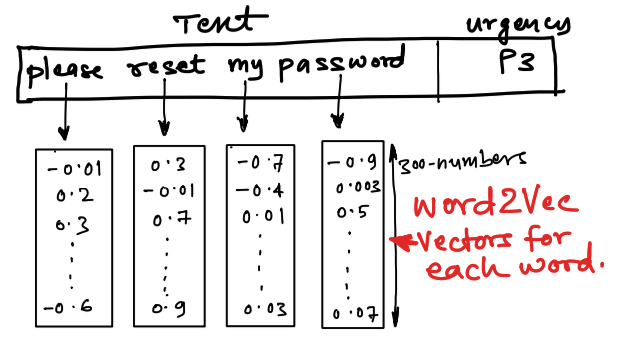
\includegraphics[width=\textwidth]{pic/word2Vec.png}
        \end{center}
    \end{columns}
\end{frame}

\begin{frame}{词向量示例——文本}
    \textbf{原始文本:}
    \begin{enumerate}
        \item "Dr.Liu always smiles, like a Angel."
        \item "Dr.Liu always encourages us."
        \item "Dr.Liu study harduous."
    \end{enumerate}

    \vspace{0.3cm}
    \textbf{词序列表示:}
    \begin{align*}
        \text{Text 1:} & [1, 2, 3, 4, 5, 6, 7] \rightarrow [0, 0, 0, 1, 2, 3, 4, 5, 6, 7] \\
        \text{Text 2:} & [1, 2, 3, 8, 9] \rightarrow [0, 0, 0, 0, 0, 1, 2, 3, 8, 9] \\
        \text{Text 3:} & [1, 2, 10, 11] \rightarrow [0, 0, 0, 0, 0, 0, 1, 2, 10, 11]
    \end{align*}
\end{frame}

\begin{frame}{词向量示例——向量}
    \vspace{0.2cm}
    \begin{center}
        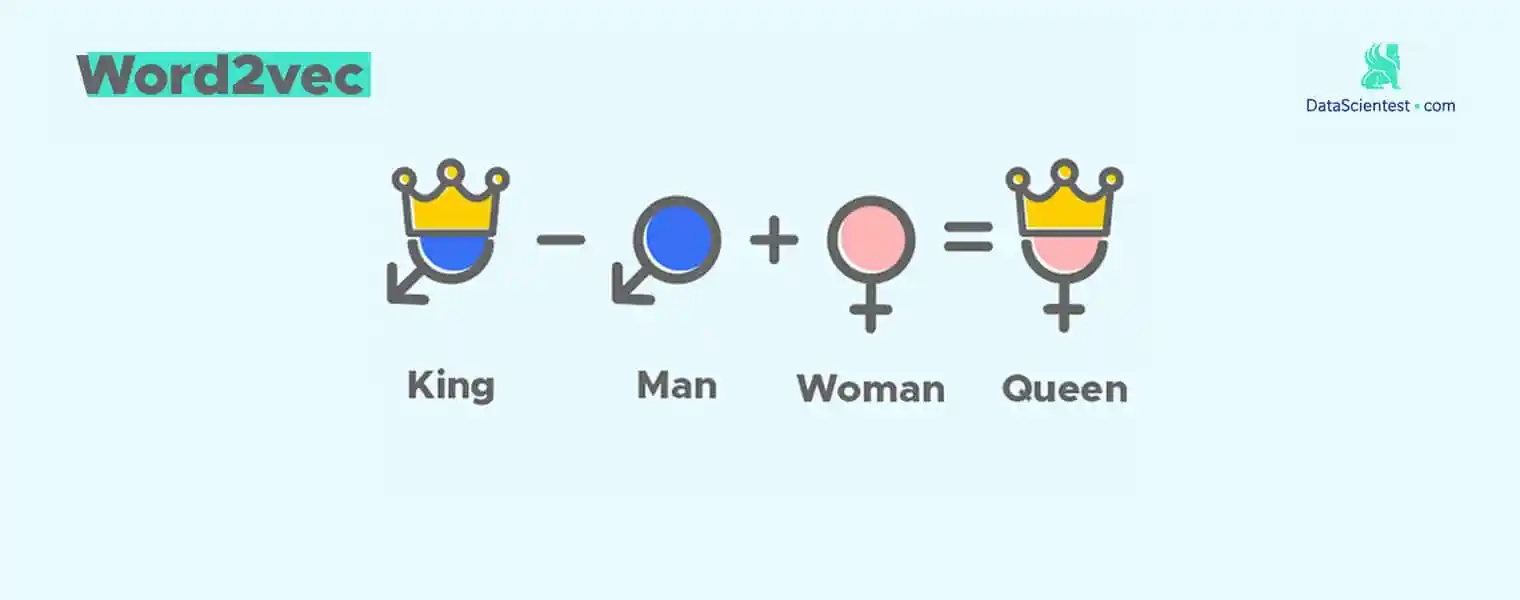
\includegraphics[width=\textwidth]{pic/word2vec2.png}
    \end{center}
    \vspace{-0.2cm}
    \begin{align*}
        \vec{v}_1 & = [ ~[0.013, -0.011, 0.039, -0.004......-0.047, 0.028, 0.025, 0.025]~ ] \\[0.2cm]
        \vec{v}_2 & = [ ~[-0.001, 0.014, 0.037, 0.003......0.001, 0.030, 0.009, 0.020]~ ] \\[0.2cm]
        \vec{v}_3 & = [ ~[-0.020, -0.008, 0.038, 0.036......-0.020, 0.043, -0.012, 0.043]~ ]
    \end{align*}
\end{frame}


% 逻辑回归涉及的特征工程是词频矩阵
\begin{frame}{逻辑回归——模型}
    \begin{columns}
        \column{0.5\textwidth}
        \textbf{模型公式}
        \begin{align*}
            P(y=1|x) & = \sigma(w^Tx + b) \\
            \sigma(z) & = \frac{1}{1 + e^{-z}}
        \end{align*}

        \vspace{0.3cm}
        \textbf{损失函数}
        \begin{equation*}
            \begin{split}
                J(w,b) = -\frac{1}{m}\sum_{i=1}^m & [y^{(i)}\log(h_{w,b}(x^{(i)})) \\
                & + (1-y^{(i)})\log(1-h_{w,b}(x^{(i)}))]
            \end{split}
        \end{equation*}

        \column{0.5\textwidth}
        \begin{tikzpicture}[scale=0.8]
            \begin{axis}[
                xlabel={$x$},
                ylabel={$y$},
                xmin=-4, xmax=4,
                ymin=-0.2, ymax=1.2,
                grid=major,
                legend pos=north west
            ]
                \addplot[red, only marks] coordinates {
                    (-3,0) (-2.5,0) (-2,0) (-1.5,0) (-1,0)
                    (1,1) (1.5,1) (2,1) (2.5,1) (3,1)
                };
                \addplot[blue, thick, smooth] {1/(1+exp(-1.5*x))};
                \addlegendentry{决策边界}
            \end{axis}
        \end{tikzpicture}
    \end{columns}
\end{frame}

\begin{frame}{逻辑回归——优化}
    \begin{columns}
        \column{0.5\textwidth}
        \textbf{梯度下降}
        \begin{align*}
            w & := w - \alpha\frac{\partial}{\partial w}J(w,b) \\
            b & := b - \alpha\frac{\partial}{\partial b}J(w,b)
        \end{align*}

        \vspace{0.3cm}
        \textbf{参数说明}
        \begin{itemize}
            \item $\alpha$: 学习率
            \item $\frac{\partial}{\partial w}J$: 损失对权重的梯度
            \item $\frac{\partial}{\partial b}J$: 损失对偏置的梯度
        \end{itemize}

        \column{0.5\textwidth}
        \begin{tikzpicture}[scale=0.8]
            \begin{axis}[
                xlabel={参数空间},
                ylabel={损失函数},
                xmin=-2, xmax=2,
                ymin=0, ymax=4,
                grid=major,
                legend pos=north east
            ]
                \addplot[blue, thick, smooth] {x^2 + 1};
                \addplot[red, ->, thick] coordinates {
                    (1.5,3.25) (1,2)
                    (0.5,1.25) (0,1)
                };
                \addlegendentry{损失曲面}
                \addlegendentry{梯度方向}
            \end{axis}
        \end{tikzpicture}
    \end{columns}
\end{frame}

\begin{frame}[fragile]{逻辑回归——模型训练}
    \begin{columns}
        \column{0.6\textwidth}
        \textbf{模型配置}
        \begin{lstlisting}[style=pythonstyle, basicstyle=\tiny]
    model = LogisticRegression(
        max_iter=1000,
        solver='liblinear'
    )
        \end{lstlisting}

        \column{0.4\textwidth}
        \begin{enumerate}
            \item \texttt{C}: 正则化强度的倒数
            \item \texttt{cv=5}: 5折交叉验证
            \item \texttt{liblinear}: 大规模文本分类
        \end{enumerate}
    \end{columns}

    % \vspace{0.2cm}
    \begin{columns}
        \column{0.6\textwidth}
        \textbf{模型训练}
        \begin{lstlisting}[style=pythonstyle, basicstyle=\tiny]
    model.compile(
        loss='binary_crossentropy',
        optimizer='adam',
        metrics=['accuracy']
    )

    history = model.fit(
        X_train_padded, y_train,
        epochs=10, batch_size=32,
        validation_split=0.2
    )
        \end{lstlisting}

        \column{0.4\textwidth}
        \begin{enumerate}
            \item 交叉熵损失函数
            \item Adam优化器自适应学习
            \item 20\%验证集划分
        \end{enumerate}
    \end{columns}
\end{frame}

\begin{frame}{逻辑回归——模型评估}
    \begin{columns}
        \column{0.6\textwidth}
        \textbf{分类报告}
        \begin{table}[h]
            \small
            \begin{tabular}{lrrr}
                \hline
                类别 & Precision & Recall & F1 \\
                \hline
                0 & 0.87 & 0.89 & 0.88 \\
                1 & 0.89 & 0.87 & 0.88 \\
                \hline
                Avg & 0.88 & 0.88 & 0.88 \\
                \hline
            \end{tabular}
        \end{table}

        \vspace{0.3cm}
        \begin{itemize}
            \item 准确率: 88\%
            \item 样本数: 25,000
            \item 正负样本均衡
        \end{itemize}

        \column{0.4\textwidth}
        \begin{center}
            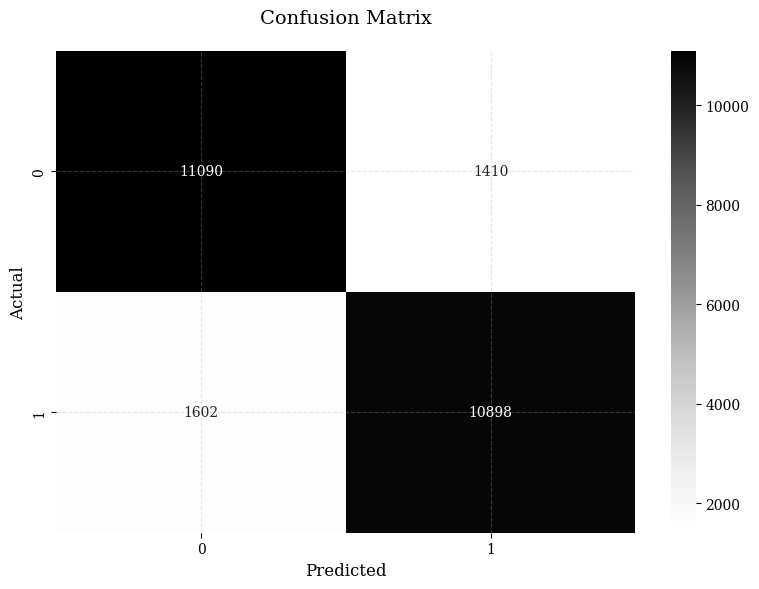
\includegraphics[width=1.3\textwidth]{pic/LR6.png}
        \end{center}
    \end{columns}
\end{frame}

\begin{frame}{逻辑回归——性能曲线}
    \begin{columns}
        \column{0.5\textwidth}
        \textbf{ROC曲线}
        \begin{center}
            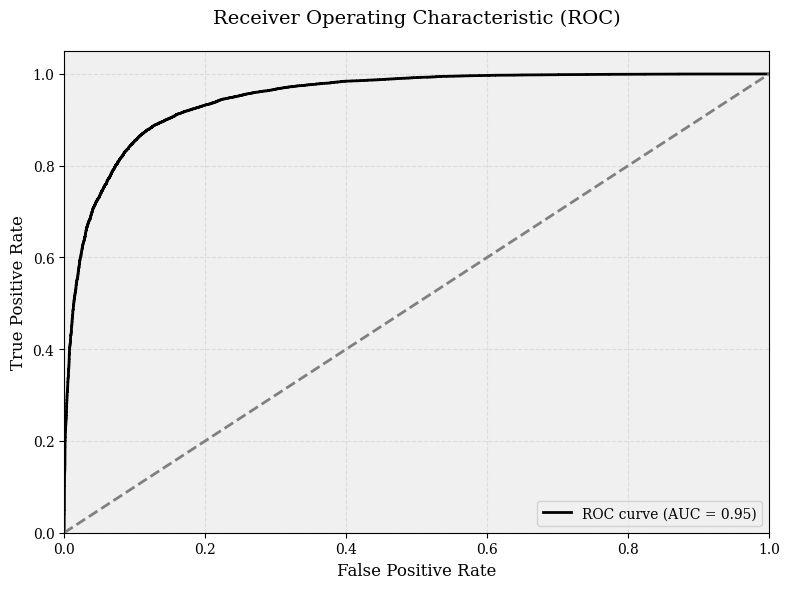
\includegraphics[width=\textwidth]{pic/LR7.png}
        \end{center}

        \column{0.5\textwidth}
        \textbf{Precision-Recall曲线}
        \begin{center}
            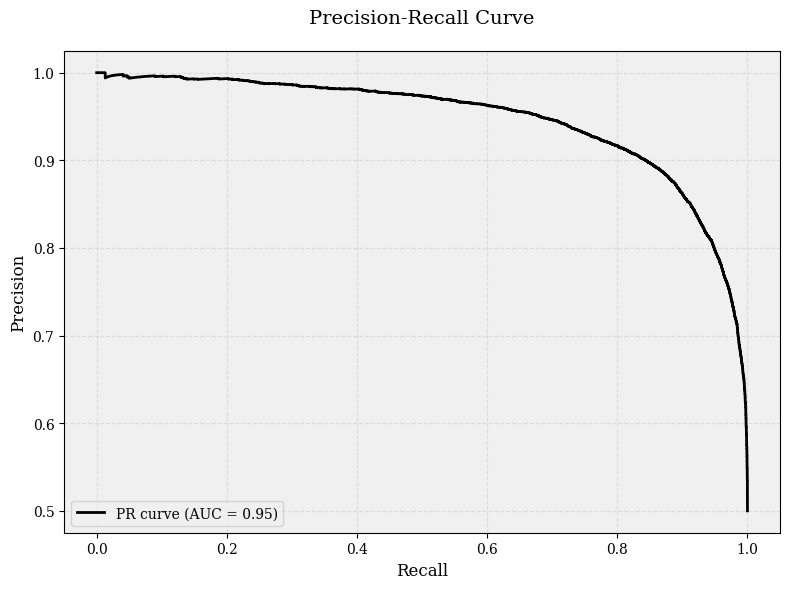
\includegraphics[width=\textwidth]{pic/LR8.png}
        \end{center}
    \end{columns}

    \begin{itemize}
        \item ROC-AUC: 衡量模型区分正负样本的能力
        \item PR曲线: 在类别不平衡时更有参考价值
    \end{itemize}
\end{frame}

\begin{frame}{特征分析——TF-IDF得分}
    \begin{columns}
        \column{0.5\textwidth}
        \textbf{特征重要性排序}
        \begin{center}
            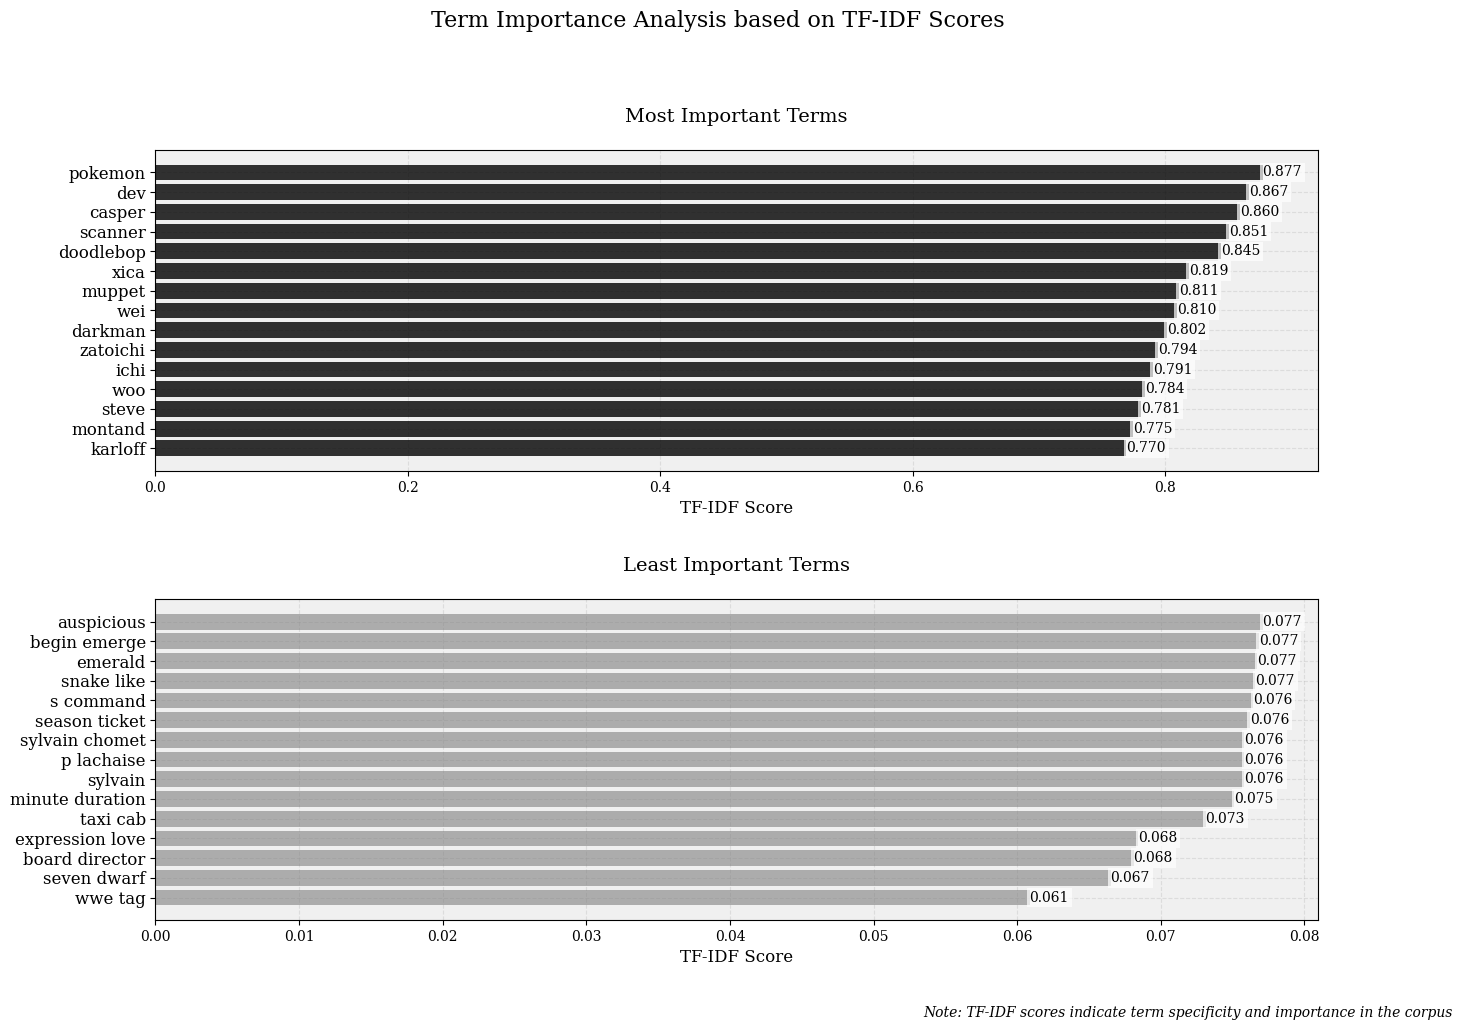
\includegraphics[width=\textwidth]{pic/LR2.png}
        \end{center}

        \column{0.5\textwidth}
        \textbf{TF-IDF词云图}
        \begin{center}
            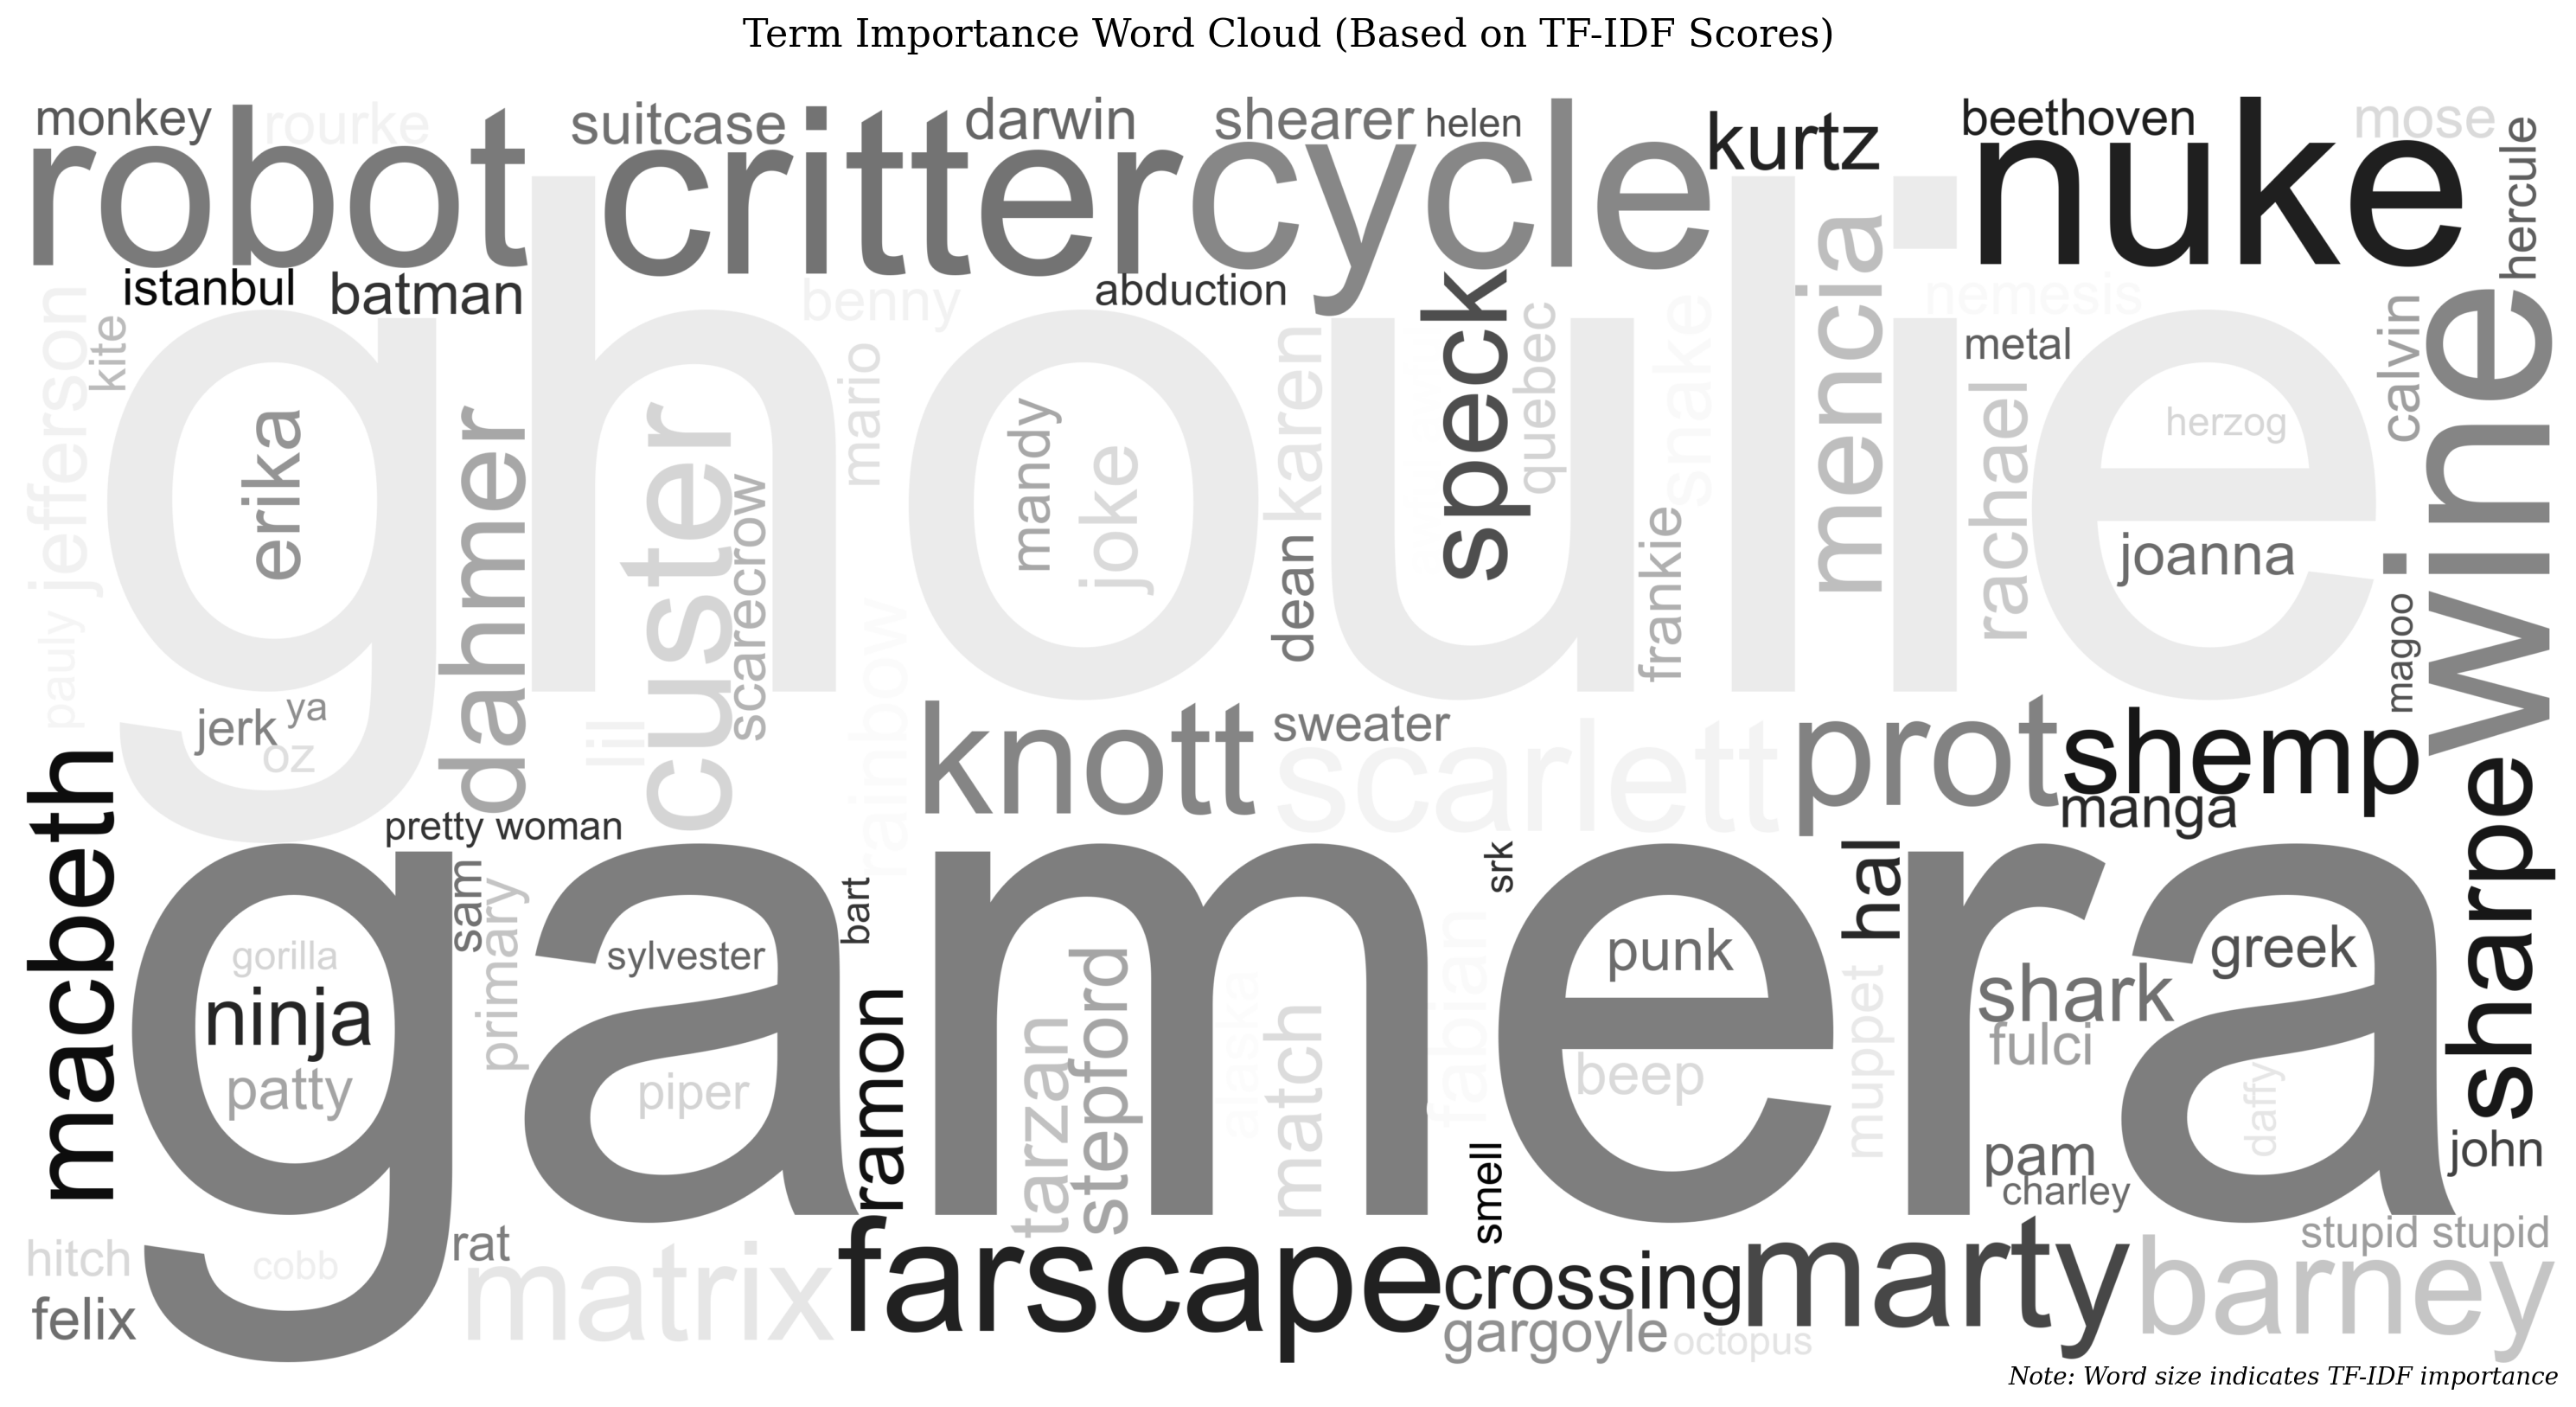
\includegraphics[width=\textwidth]{pic/LR3.png}
        \end{center}
    \end{columns}
    \vspace{0.2cm}
    \begin{enumerate}
        \item 横向条形图显示各词的TF-IDF得分
        \item 词云直观展示高频重要词汇
    \end{enumerate}
\end{frame}

\begin{frame}{特征分析——模型系数}
    \begin{columns}
        \column{0.5\textwidth}
        \textbf{系数条形图}
        \begin{center}
            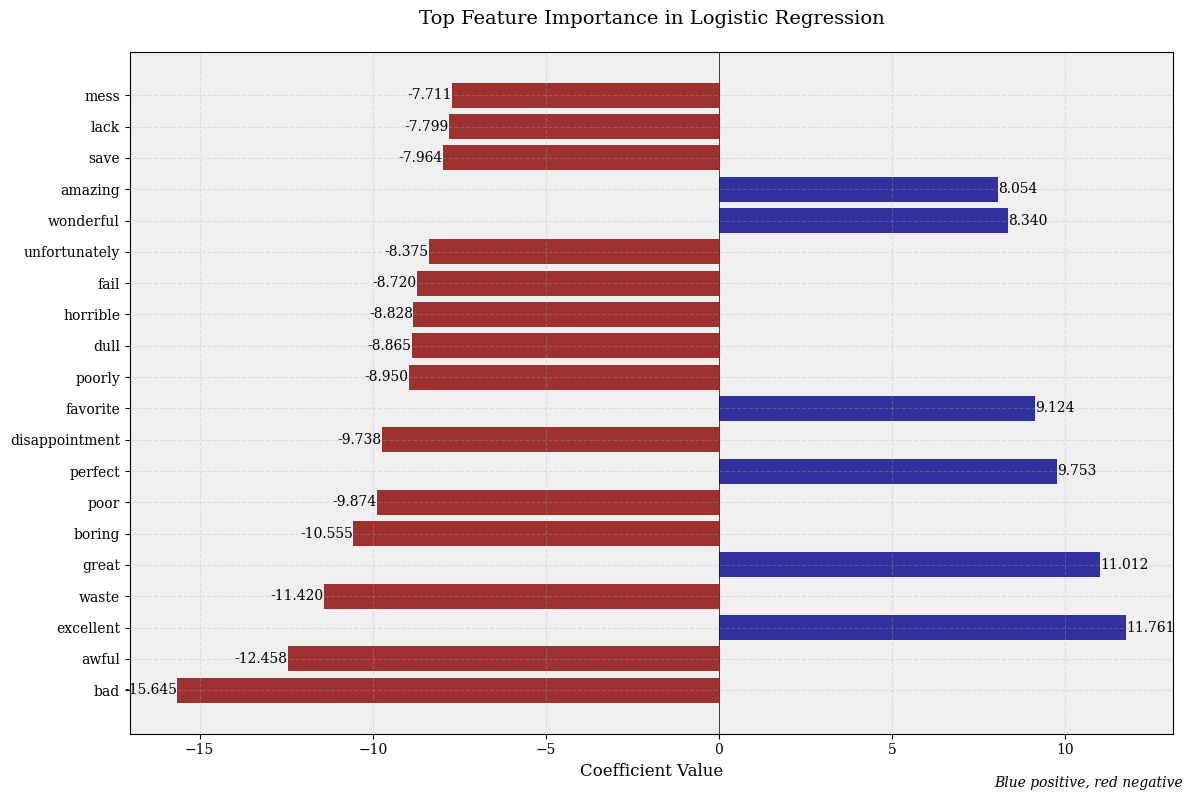
\includegraphics[width=\textwidth]{pic/LR4.png}
        \end{center}

        \column{0.5\textwidth}
        \textbf{评论词云图}
        \begin{center}
            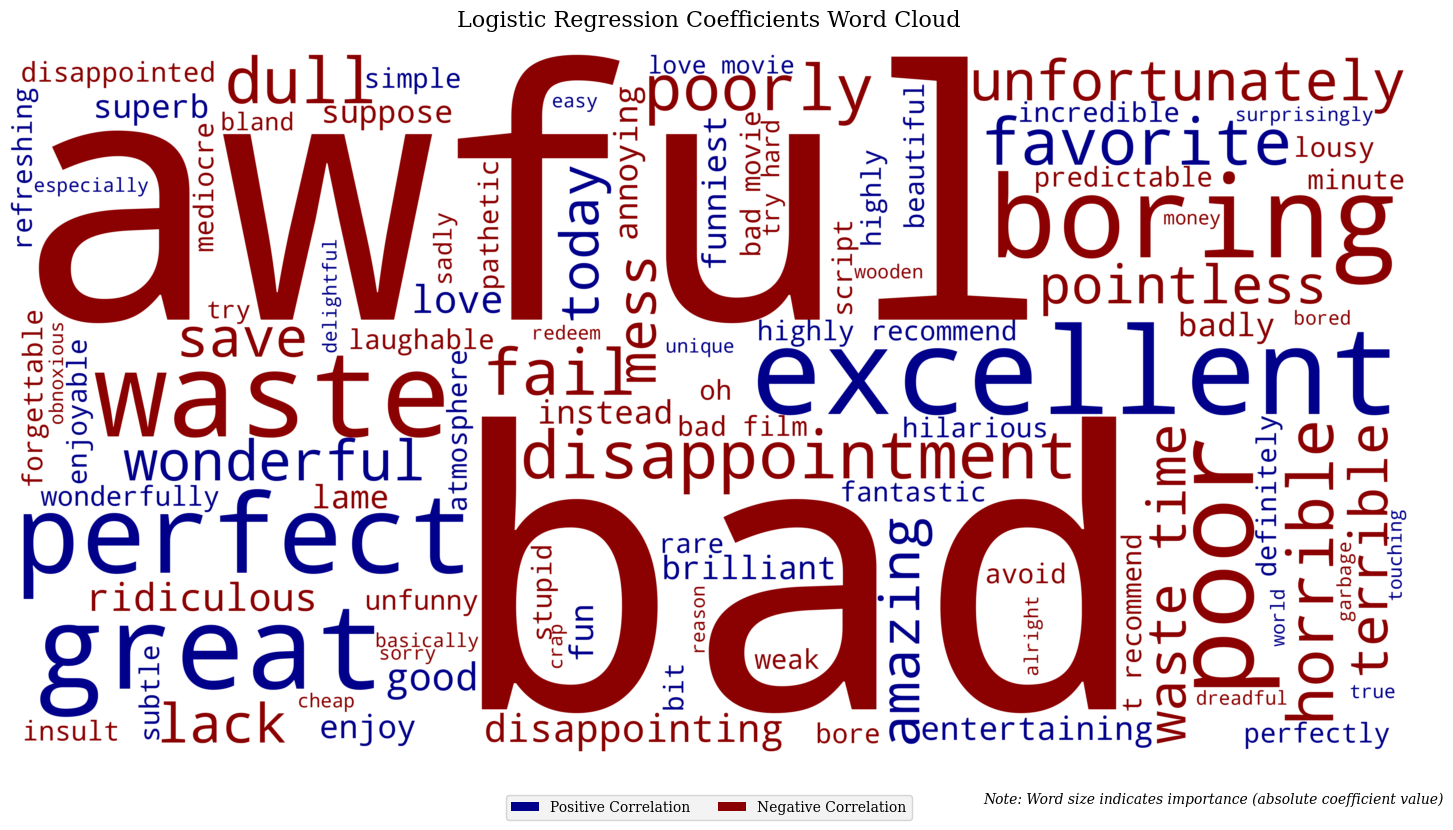
\includegraphics[width=\textwidth]{pic/LR5.png}
        \end{center}
    \end{columns}
    \vspace{0.2cm}
    \begin{enumerate}
        \item 横向条形图显示各词的系数
        \item 词云直观展示高频重要词汇
    \end{enumerate}
\end{frame}

% LSTM涉及的特征工程是词向量 Word2Vec
\begin{frame}{LSTM}
    \begin{center}
        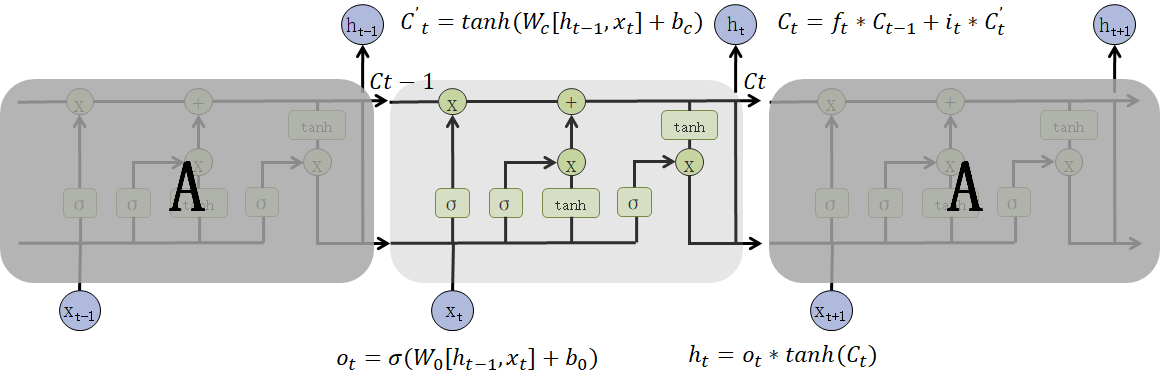
\includegraphics[width=\textwidth]{pic/LSTM.png}
    \end{center}

    \vspace{0.2cm}
    \begin{columns}
        \column{0.5\textwidth}
        \textbf{门控机制}
        \begin{align*}
            f_t & = \sigma(W_f \cdot [h_{t-1}, x_t] + b_f) \\
            i_t & = \sigma(W_i \cdot [h_{t-1}, x_t] + b_i) \\
            o_t & = \sigma(W_o \cdot [h_{t-1}, x_t] + b_o)
        \end{align*}

        \column{0.5\textwidth}
        \textbf{状态更新}
        \begin{align*}
            \tilde{C}_t & = \tanh(W_c \cdot [h_{t-1}, x_t] + b_c) \\
            C_t & = f_t \odot C_{t-1} + i_t \odot \tilde{C}_t \\
            h_t & = o_t \odot \tanh(C_t)
        \end{align*}
    \end{columns}

\end{frame}

\begin{frame}[fragile]{LSTM——模型训练}
    \begin{columns}
        \column{0.6\textwidth}
        \textbf{模型构建}
        \begin{lstlisting}[style=pythonstyle, basicstyle=\tiny]
    model = Sequential()
    model.add(Embedding(
        input_dim=vocab_size,
        output_dim=128,
        weights=[embedding_matrix],
        trainable=False
    ))
    model.add(Bidirectional(LSTM(64)))
    model.add(Dropout(0.5))
    model.add(Dense(1, activation='sigmoid'))
        \end{lstlisting}

        \column{0.4\textwidth}
        \begin{enumerate}
            \item 词嵌入层固定权重
            \item 双向LSTM捕捉上下文
            \item Dropout防止过拟合
        \end{enumerate}
    \end{columns}

    % \vspace{0.2cm}
    \begin{columns}
        \column{0.6\textwidth}
        \textbf{模型训练}
        \begin{lstlisting}[style=pythonstyle, basicstyle=\tiny]
    model.compile(
        loss='binary_crossentropy',
        optimizer='adam',
        metrics=['accuracy']
    )

    history = model.fit(
        X_train_padded, y_train,
        epochs=10, batch_size=32,
        validation_split=0.2
    )
        \end{lstlisting}

        \column{0.4\textwidth}
        \begin{enumerate}
            \item 交叉熵损失函数
            \item Adam优化器自适应学习
            \item 20\%验证集划分
        \end{enumerate}
    \end{columns}
\end{frame}

\begin{frame}{LSTM——训练结果}
    \begin{columns}
        \column{0.5\textwidth}
        \begin{table}
            \begin{tabular}{cccc}
                \hline
                Epoch & Loss & Accuracy & Val Acc \\
                \hline
                1 & 0.631 & 0.651 & 0.688 \\
                2 & 0.484 & 0.782 & 0.822 \\
                3 & 0.352 & 0.853 & 0.863 \\
                ... & ... & ... & ... \\
                8 & 0.269 & 0.890 & 0.884 \\
                9 & 0.264 & 0.892 & 0.862 \\
                10 & 0.254 & 0.897 & 0.882 \\
                \hline
            \end{tabular}
        \end{table}
        \vspace{0.3cm}
        \begin{enumerate}
            \item 最终测试准确率: 88.24\%
            \item 训练时间: 约35s/epoch
            \item 最终准确率基于测试集
        \end{enumerate}

        \column{0.5\textwidth}
        \begin{figure}
            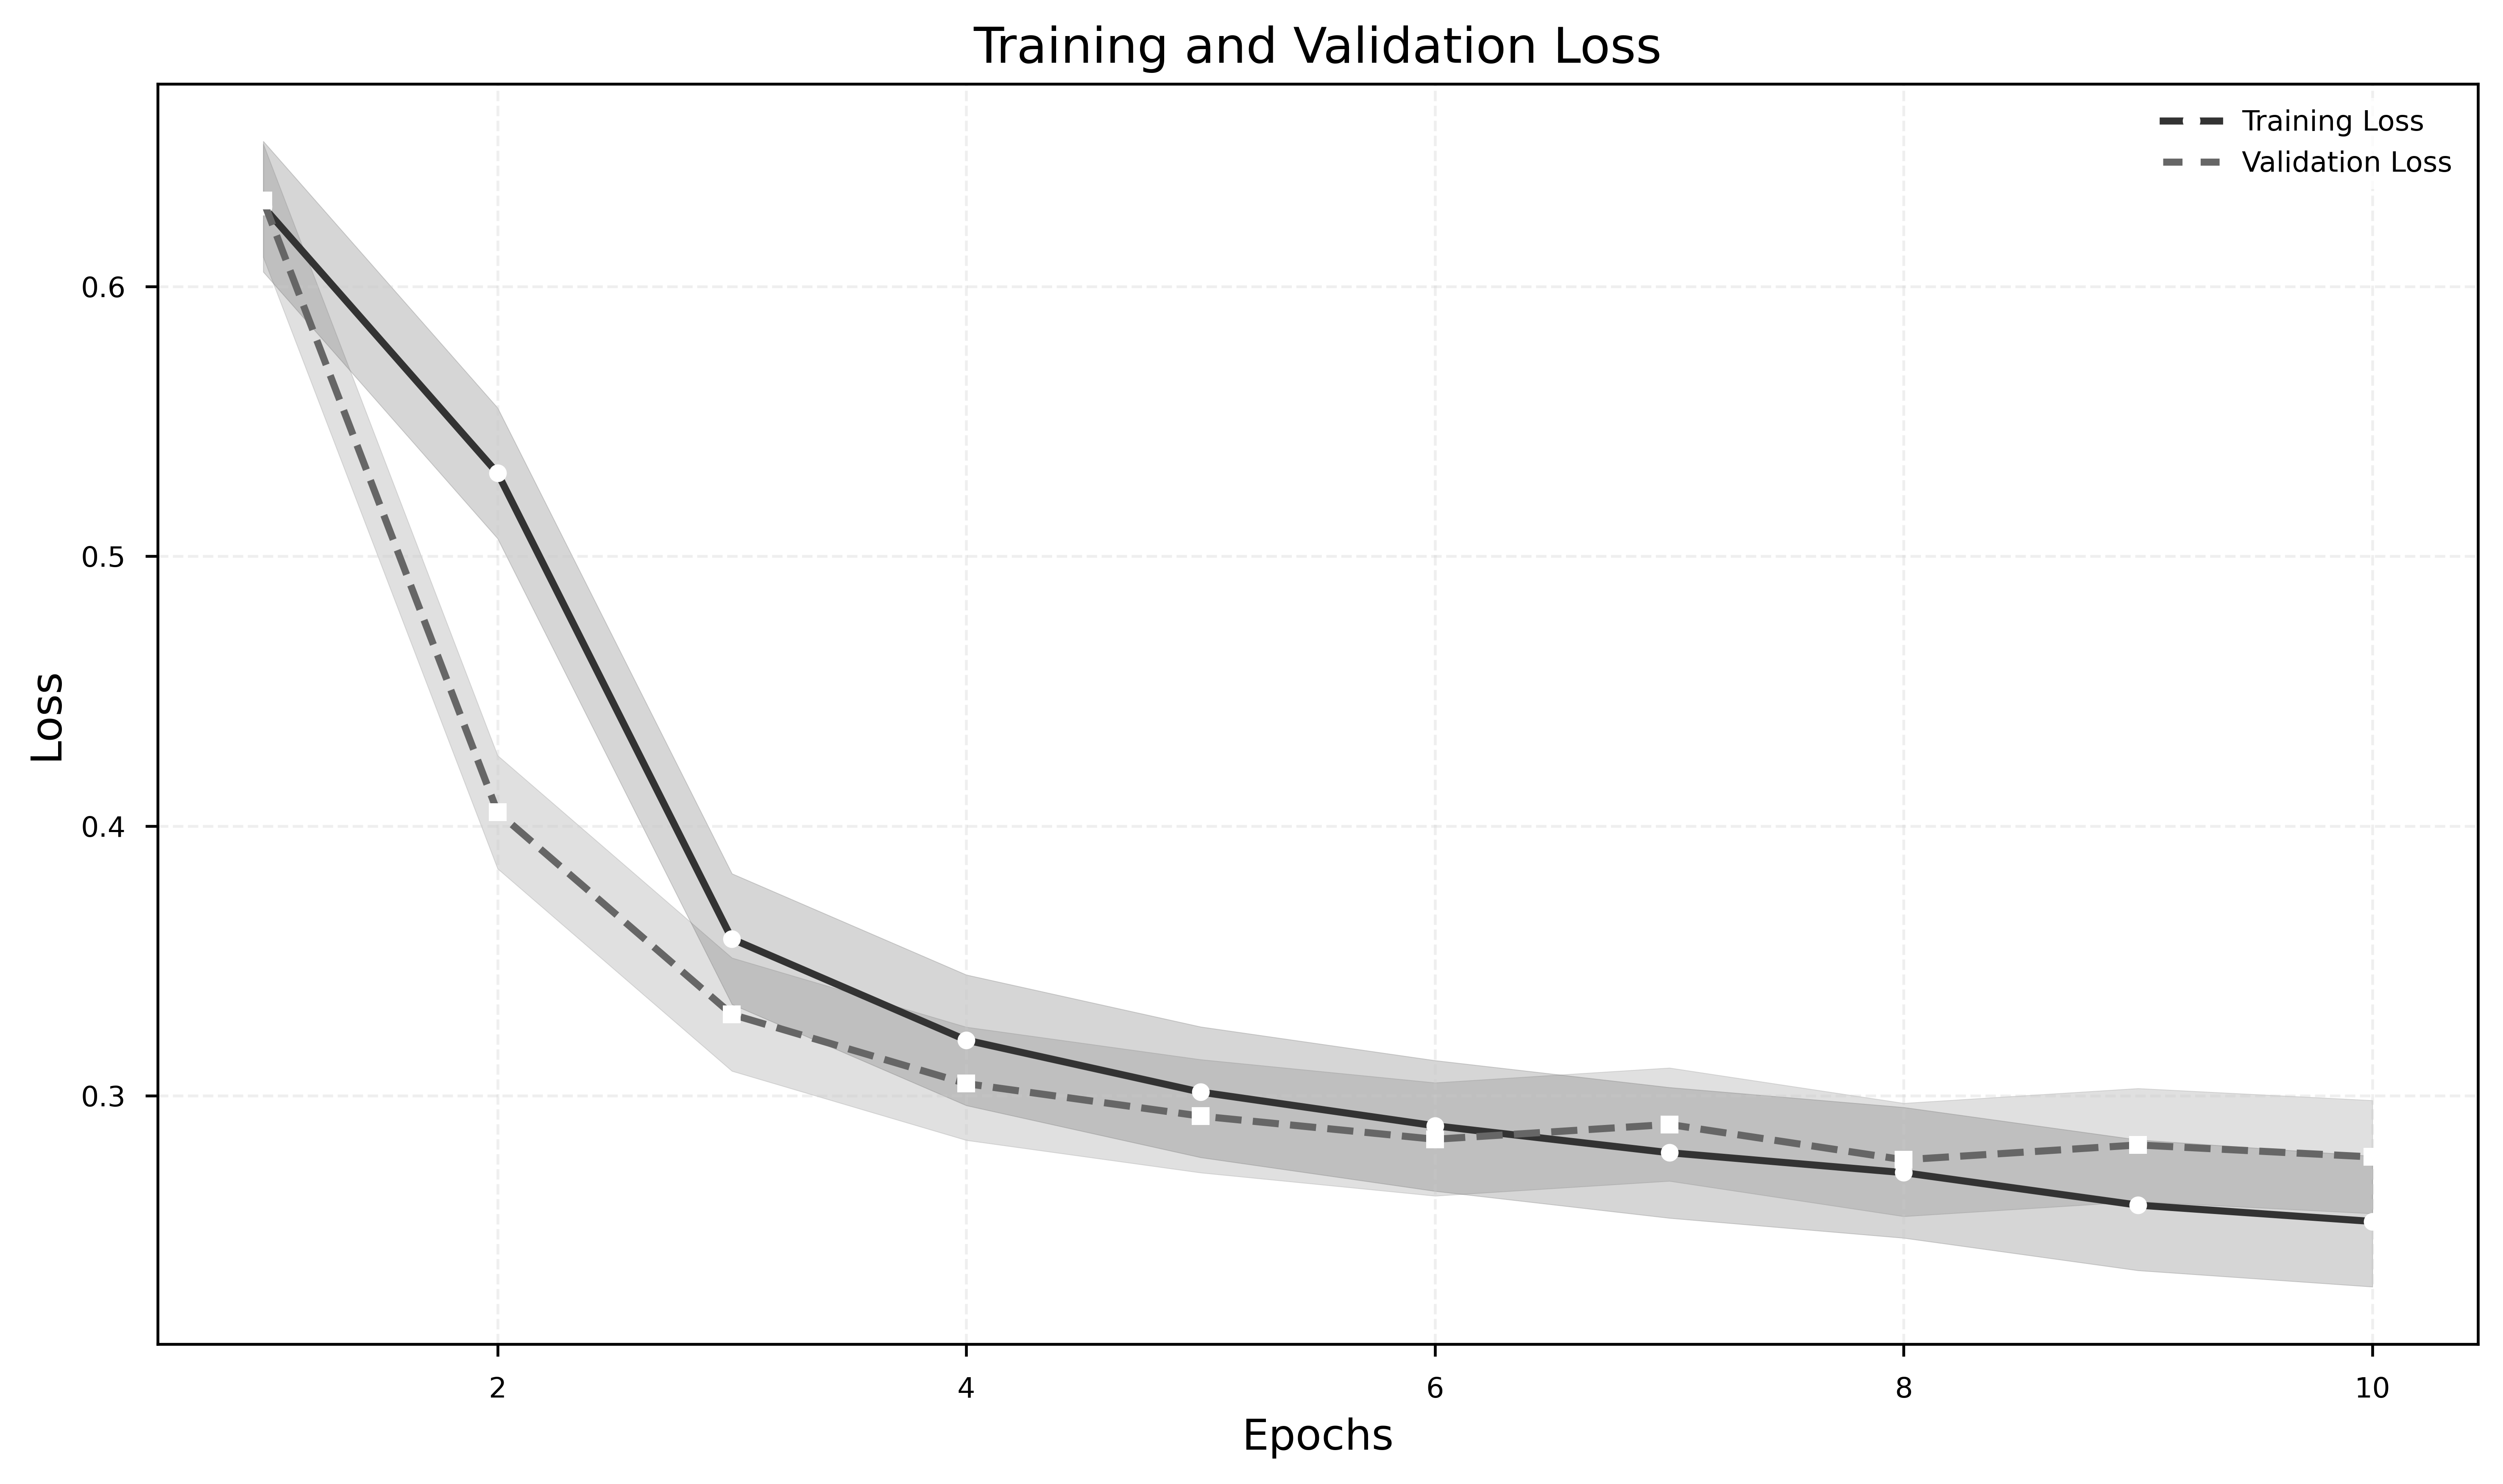
\includegraphics[width=\textwidth]{pic/LSTM1.png}
            \vspace{0.2cm}
            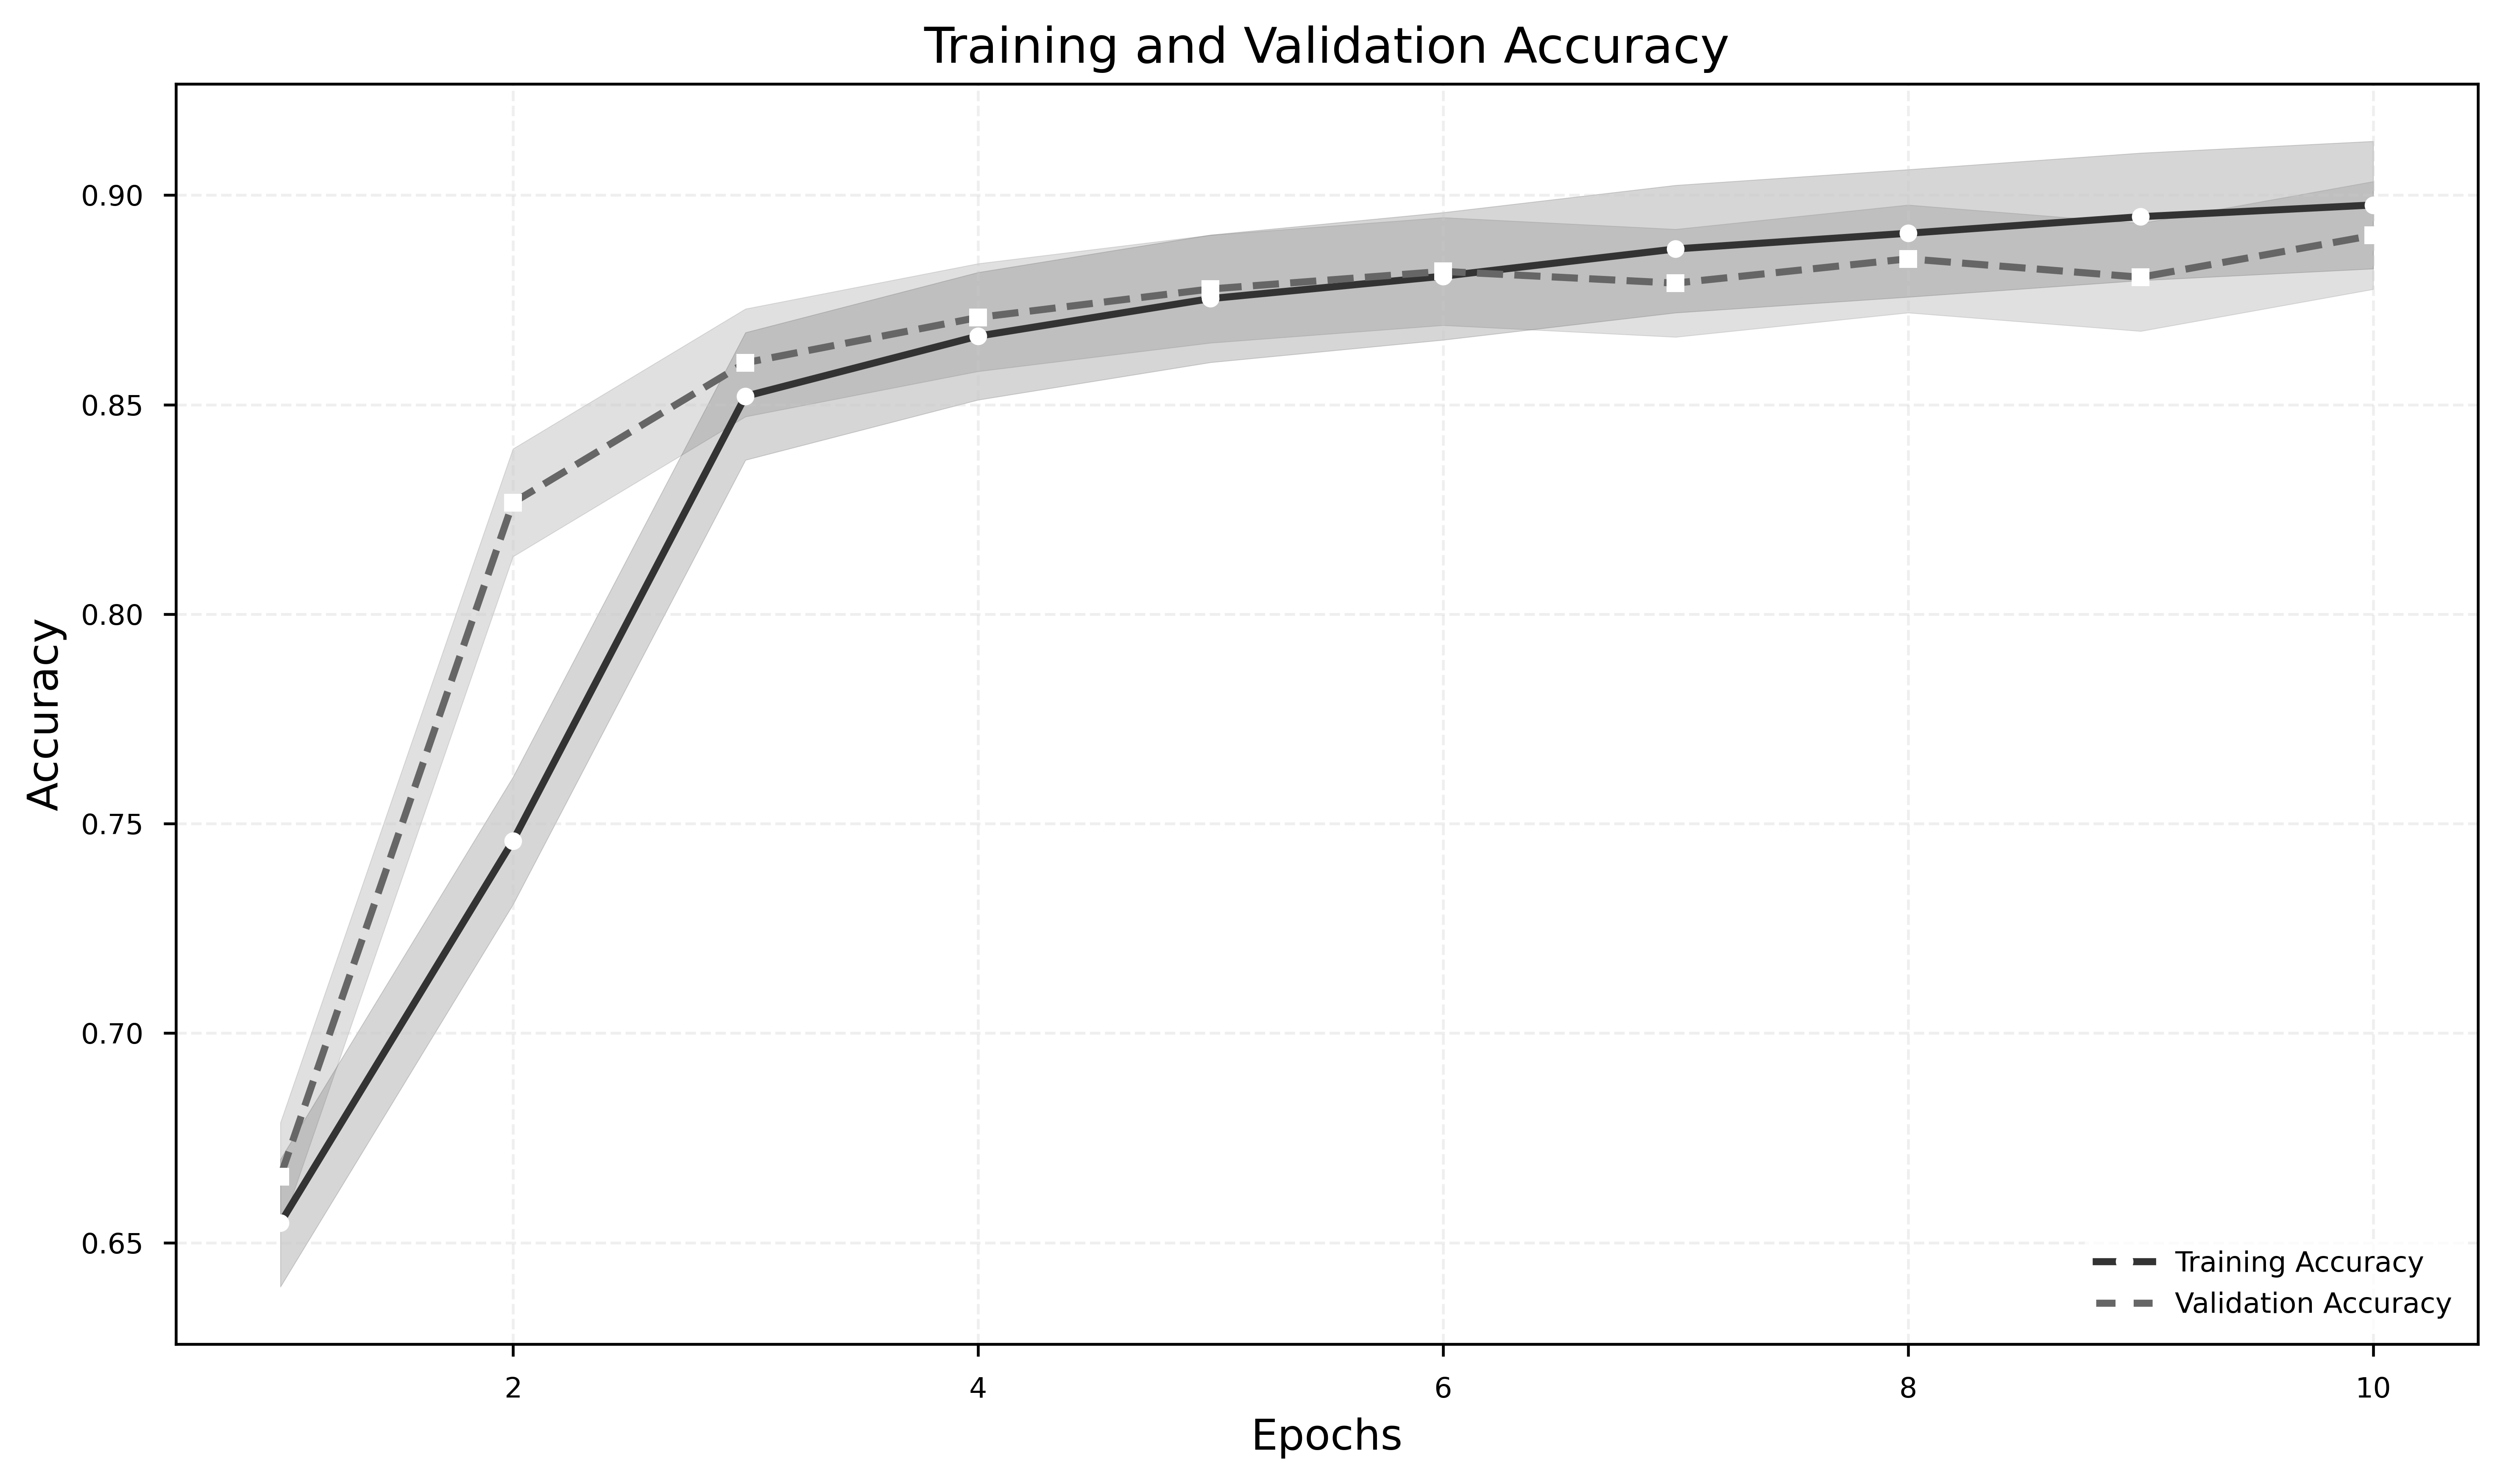
\includegraphics[width=\textwidth]{pic/LSTM2.png}
        \end{figure}
    \end{columns}
\end{frame}

\begin{frame}[fragile]{LR-LSTM模型融合——权重学习}
    \begin{columns}[T]
        \column{0.5\textwidth}
        \begin{algorithm}[H]
        \scriptsize
        \caption{Learn Ensemble Weights}
        \begin{algorithmic}[1]
        \STATE \textbf{Input:} validation dataset $D_{val}$
        \STATE \textbf{Output:} optimal weights $w_{lr}, w_{lstm}$
        \STATE Load pre-trained models $M_{lr}, M_{lstm}$
        \STATE $best\_acc \gets 0$
        \FOR{$w \gets 0$ to $1.0$ step $0.05$}
            \STATE $acc \gets accuracy(Y_{true}, (w \cdot M_{lr} + (1-w) \cdot M_{lstm}).predict\_proba(D_{val}) \geq 0.5)$
            \IF{$acc > best\_acc$}
                \STATE $best\_acc \gets acc$
                \STATE $w_{lr} \gets w$
            \ENDIF
        \ENDFOR
        \STATE $w_{lstm} \gets 1 - w_{lr}$
        \STATE \RETURN $w_{lr}, w_{lstm}$
        \end{algorithmic}
        \end{algorithm}
        
        \column{0.5\textwidth}
        \vspace{0.5cm}
        \textbf{权重学习策略:}
        \begin{itemize}
            \item 使用验证集(review\_polarity)评估不同权重组合
            \item 网格搜索最优权重配比
            \item 优化目标:最大化准确率
            \item 权重和为1,确保概率有效
        \end{itemize}
    \end{columns}
\end{frame}

\begin{frame}[fragile]{LR-LSTM模型融合——预测}
    \begin{columns}[T]
        \column{0.5\textwidth}
        \begin{algorithm}[H]
        \scriptsize
        \caption{Ensemble Prediction}
        \begin{algorithmic}[1]
        \STATE \textbf{Input:} text $T$, weights $w_{lr}, w_{lstm}$
        \STATE \textbf{Output:} predicted sentiment and topic
        \STATE $p_{lr} \leftarrow$ LR.predict($T$)
        \STATE $p_{lstm} \leftarrow$ LSTM.predict($T$)
        \STATE $sentiment \leftarrow w_{lr} \cdot p_{lr} + w_{lstm} \cdot p_{lstm}$
        \STATE \textbf{if} $sentiment > 0.5$ \textbf{then}
        \STATE \quad return positive
        \STATE \textbf{else}
        \STATE \quad return negative
        \STATE \textbf{end if}
        \end{algorithmic}
        \end{algorithm}
        
        \column{0.5\textwidth}
        \vspace{0.5cm}
        \textbf{模型融合优势:}
        \begin{itemize}
            \item 结合两个模型的优势
            \item LR模型:特征解释性强
            \item LSTM模型:捕捉序列特征
            \item 加权平均:平滑预测结果
            \item 准确率提升到90\%
        \end{itemize}
    \end{columns}
\end{frame}

\section{无监督学习}

\begin{frame}[fragile]{LDA——潜在狄利克雷分配}
    \begin{columns}
        \column{0.5\textwidth}
        \textbf{文档生成过程:}
        \vspace{0.2cm}
        \begin{enumerate}
            \item 按照先验概率$p(d_i)$选择一篇文档$d_i$
            \item 从Dirichlet分布$\alpha$中取样生成文档$d_i$的主题分布$\theta_i$
            \item 从主题的多项式分布$\theta_i$中取样生成文档$d_i$第j个词的主题$z_{i,j}$
            \item 从Dirichlet分布$\beta$中取样生成主题$z_{i,j}$对应的词语分布$\phi_{z_{i,j}}$
            \item 从词语的多项式分布$\phi_{z_{i,j}}$中采样最终生成词语$\omega_{i,j}$
        \end{enumerate}

        \column{0.5\textwidth}
        \textbf{模型实现:}
        \begin{lstlisting}[style=pythonstyle, basicstyle=\tiny]
    lda = LatentDirichletAllocation(
        n_components=15,
        max_iter=5,
        learning_method='online',
        learning_offset=50.,
        random_state=0
    )
    lda.fit(X)
        \end{lstlisting}
        \vspace{0.2cm}
        \textbf{参数说明:}
        \begin{itemize}
            \item n\_components: 主题数量
            \item max\_iter: 最大迭代次数
            \item learning\_method: 在线学习
            \item learning\_offset: 学习率参数
        \end{itemize}
    \end{columns}
\end{frame}

\begin{frame}{LDA——主题分布}
    \begin{columns}
        \column{0.5\textwidth}
        \textbf{15个主题类别:}
        \begin{description}
            \item[观后感] thought, thing, lot...
            \item[音乐舞蹈] music, musical, songs...
            \item[喜剧] comedy, funny, fun...
            \item[表演] role, performance, cast...
            \item[社会议题] sex, women, american...
            \item[恐怖] horror, effects, gore...
        \end{description}

        \column{0.5\textwidth}
        \begin{figure}
            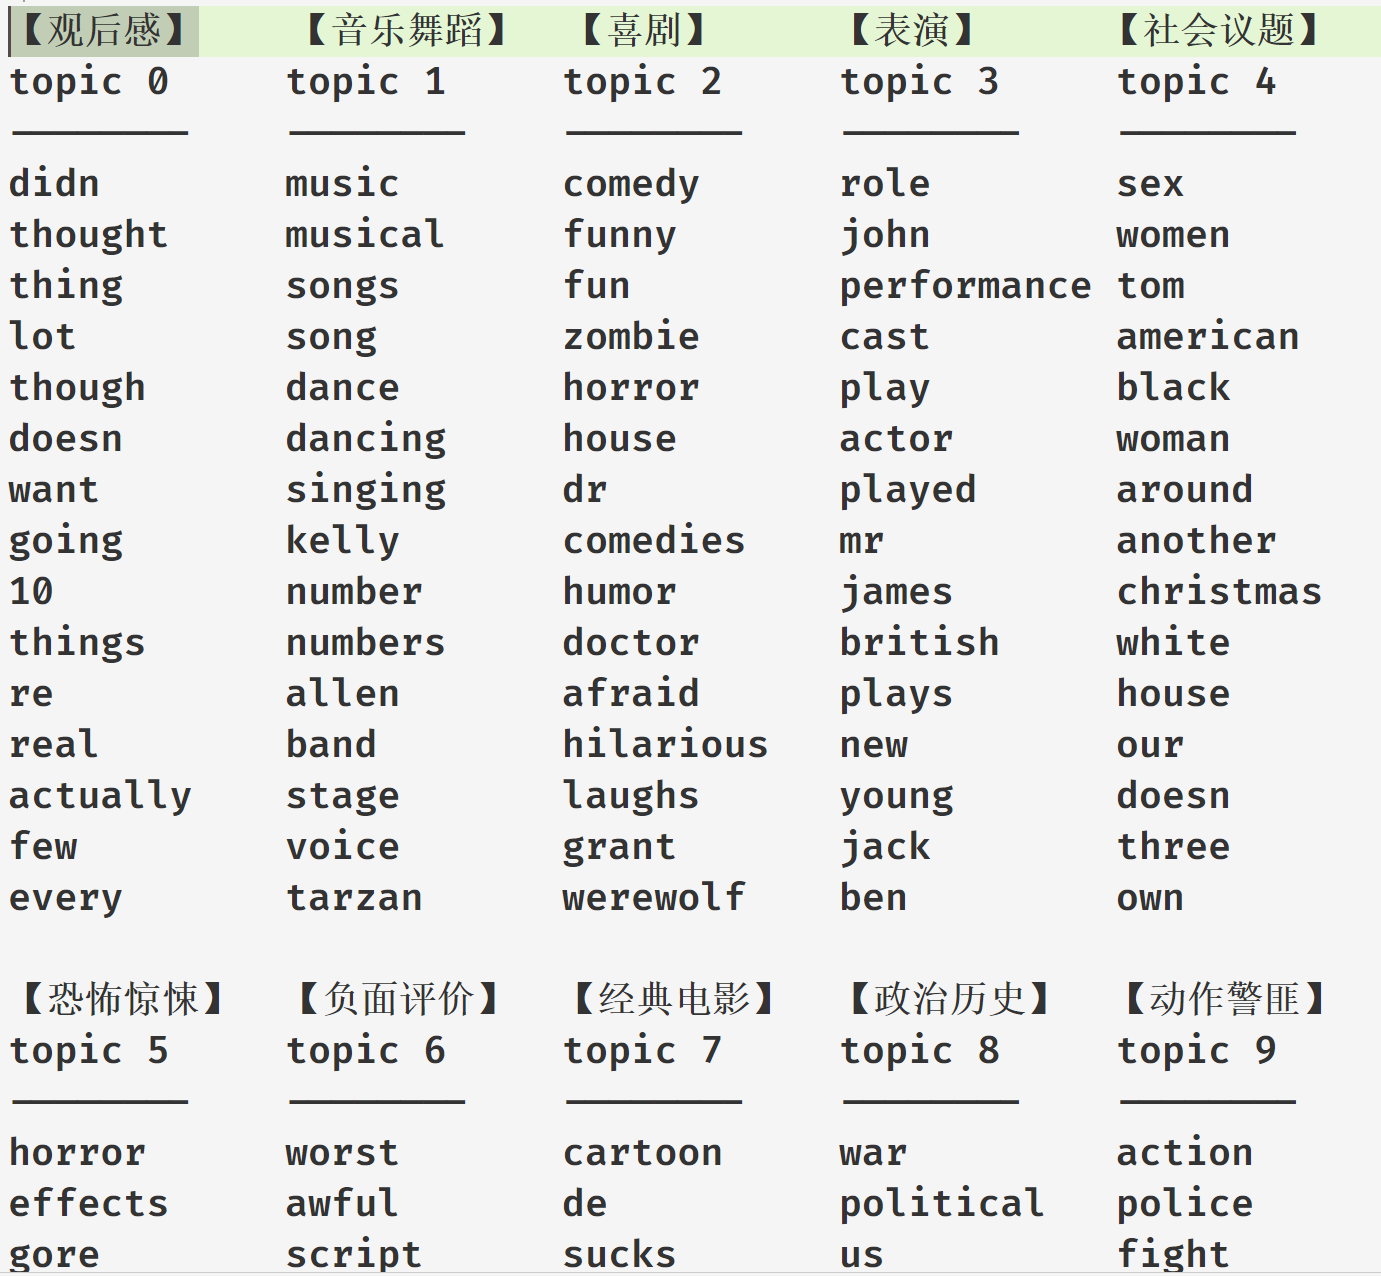
\includegraphics[width=\textwidth]{pic/topic.png}
        \end{figure}
    \end{columns}
\end{frame}

\begin{frame}{LDA——文档-主题矩阵}
    \begin{columns}
        \column{0.5\textwidth}
        \textbf{矩阵结构:}
        \begin{itemize}
            \item 行: 每一行代表一条文本
            \item 列: 每一列代表一个主题
            \item 值: 文本属于该主题的概率
        \end{itemize}
        \vspace{0.3cm}
        \textbf{矩阵特点:}
        \begin{itemize}
            \item 概率和为1
            \item 反映文本的主题分布
            \item 可用于文本分类和聚类
        \end{itemize}

        \column{0.5\textwidth}
        \begin{center}
            \begin{tabular}{cccc}
                \hline
                 & 观后感 & 音乐舞蹈 & ... \\
                \hline
                T1 & p11 & p12 & ... \\
                T2 & p21 & p22 & ... \\
                T3 & p31 & p32 & ... \\
                ... & ... & ... & ... \\
                \hline
            \end{tabular}
        \end{center}
    \end{columns}
\end{frame}


\section{模型应用}

\begin{frame}[fragile]{后端接口一:情感分析}
    \begin{columns}
        \column{0.5\textwidth}
        \textbf{接口说明:}
        \begin{itemize}
            \item 路由: \texttt{/api/sentiment}
            \item 方法: \texttt{POST}
            \item 功能: 融合LR和LSTM的情感分析
        \end{itemize}
        \vspace{0.2cm}
        \textbf{特点:}
        \begin{itemize}
            \item 模型融合: LR权重0.6, LSTM权重0.4
            \item 文本预处理: 清洗、分词、序列化
            \item 返回详细概率分布
        \end{itemize}

        \column{0.5\textwidth}
        \textbf{返回示例:}
        \begin{lstlisting}[style=pythonstyle, basicstyle=\tiny]
    {
        "sentiment": "positive",
        "probability": 0.85,
        "model_details": {
            "logistic_regression_prob": 0.82,
            "lstm_prob": 0.89
        }
    }
        \end{lstlisting}
    \end{columns}
\end{frame}

\begin{frame}[fragile]{后端接口二:主题分类}
    \begin{columns}
        \column{0.5\textwidth}
        \textbf{接口说明:}
        \begin{itemize}
            \item 路由: \texttt{/api/topic}
            \item 方法: \texttt{POST}
            \item 功能: LDA主题分布分析
        \end{itemize}
        \vspace{0.2cm}
        \textbf{特点:}
        \begin{itemize}
            \item 15个预定义主题
            \item 返回完整主题分布
            \item 主题映射转换
        \end{itemize}

        \column{0.5\textwidth}
        \textbf{返回示例:}
        \begin{lstlisting}[style=pythonstyle, basicstyle=\tiny]
    {
        "topic": "music and dance",
        "topic_id": 1,
        "confidence": 0.75,
        "topic_distribution": {
            "0": 0.1,
            "1": 0.75,
            "2": 0.15
        }
    }
        \end{lstlisting}
    \end{columns}
\end{frame}

\begin{frame}[fragile]{后端接口三:智能分析集成}
    \begin{columns}
        \column{0.4\textwidth}
        \textbf{接口说明:}
        \begin{itemize}
            \item 路由: \texttt{/api/analyze}
            \item 方法: \texttt{POST}
            \item 功能: 模型预测 + GPT分析
        \end{itemize}
        \vspace{0.2cm}
        \textbf{创新设计:}
        \begin{enumerate}
            \item 模型预测结果(情感/主题)作为GPT输入
            \item 定制化prompt引导分析
            \item 结构化输出集成
        \end{enumerate}

        \column{0.6\textwidth}
        \begin{tikzpicture}[font=\small]
            \tikzstyle{entity} = [draw, rectangle, minimum height=1em]
            
            % 定义实体
            \node[entity] (front) at (0,4) {前端};
            \node[entity] (api) at (2,4) {API};
            \node[entity] (models) at (4,4) {模型(double)};
            \node[entity] (gpt) at (6,4) {GPT};
            
            % 绘制生命线
            \draw[dashed] (front) -- (0,0);
            \draw[dashed] (api) -- (2,0);
            \draw[dashed] (models) -- (4,0);
            \draw[dashed] (gpt) -- (6,0);
            
            % 绘制消息
            \draw[->] (0,3.5) -- (2,3.5) node[midway,above] {文本};
            \draw[->] (2,3) -- (4,3) node[midway,above] {预测请求};
            \draw[->] (4,2.5) -- (2,2) node[midway,above] {预测结果};
            \draw[->] (2,1.5) -- (6,1.5) node[midway,above] {构建prompt};
            \draw[->] (6,1) -- (2,1) node[midway,above] {分析结果};
            \draw[->] (2,0.5) -- (0,0.5) node[midway,above] {JSON响应};
        \end{tikzpicture}
    \end{columns}
\end{frame}



\begin{frame}{前端应用}
    \begin{columns}[T]
        \column{0.4\textwidth}
        \textbf{技术栈:}
        \begin{itemize}
            \item React + Vite
            \item TailwindCSS
            \item Modern ES6+
        \end{itemize}
        \vspace{0.3cm}
        \textbf{主要组件:}
        \begin{itemize}
            \item ChatArea: 对话展示
            \item InputArea: 用户输入
            \item ChatMessage: 消息气泡
            \item Header: 导航与功能
        \end{itemize}
        
        \column{0.6\textwidth}
        \vspace{-0.5cm}
        \begin{figure}
            
\includegraphics[width=0.49\textwidth]{pic/front1.png}
            
\includegraphics[width=0.49\textwidth]{pic/front2.png}
        \end{figure}
    \end{columns}
\end{frame}

\begin{frame}{App应用}
    \begin{columns}[T]
        \column{0.5\textwidth}
        \begin{figure}
            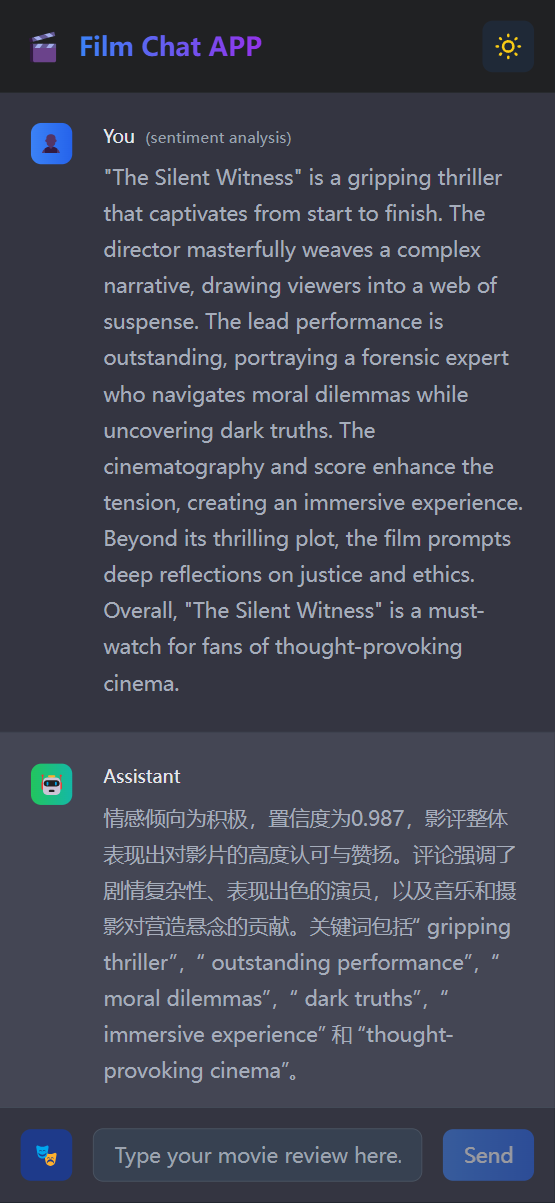
\includegraphics[width=\textwidth,height=0.7\textheight,keepaspectratio]{pic/display1.png}
            \centering
            \\
            \small{展示积极/消极概率分布}
        \end{figure}
        
        \column{0.5\textwidth}
        \begin{figure}
            
\includegraphics[width=\textwidth,height=0.7\textheight,keepaspectratio]{pic/display2.png}
            \centering
            \\
            \small{显示主题分布情况}
        \end{figure}
    \end{columns}
\end{frame}

\begin{frame}
    \begin{center}
        {\Huge\calligra Thanks}
        % {\Huge\calligra 教会学成、守正有为}
    \end{center}
\end{frame}

\end{document}